Supppose we are given
%\begin{multicols}{2}
\begin{itemize}
	\item binary columns $\bit{1}$, $\bit{2}$ and $\bit{3}$,
	\item counter-constant columns  \source{}, \target{},
	\item a byte column \source{}\byte{},
	\item counter-constant columns \source{}\mark{} and \size{},
	\item an ``accumulator column'' \ACC{},
	\item a ``power''column \col{P},
	\item a ``counter column'' \ct{}.
	%\item[\vspace{\fill}]
\end{itemize}
%\end{multicols}
The interpretation is as follows:
\source{} is a limb from which we will harvest a chunk of bytes;
\source{}\byte{} is the byte decomposition of \source{};
\source{}\mark{} is the offset within \source{} from where we start harvesting bytes;
\size{} is the number of bytes to harvest;
the assumption is that $\source{}\mark{} + (\size{}-1) \leq \llargeMO$;
\target{} will be made to contain this chunk of bytes (left aligned);
$\bit{1}$ plateaus at \source{}\mark{};
$\bit{2}$ plateaus at $\source{}\mark{} + \size{}$;
$\bit{3}$ plateaus at $\size{}$;
$\col{P}$ is pegged to $\bit{3}$ and builds the correct power of $256$ so that we may shift the harvested chunk to build the desired (left-aligned) prefix.
Compare with figure~\ref{fig: one partial to one padded}

We the following collection of constraints ensures the desired behaviour:
\begin{enumerate}
	\item binary plateau constraints:
	\begin{enumerate}
		\item $\plateau(\bit{1}, \source{}\mark{}; \ct{})$,
		\item $\plateau(\bit{2}, \source{}\mark{} + \size{}; \ct{})$,
		\item $\plateau(\bit{3}, \size{}; \ct{})$;
	\end{enumerate}
	\item chunk constraint: $\compChunk(\ACC{}, \source{}\byte{}, \bit{1}, \bit{2}; \ct{})$;
	\item power constraint: $\power(\col{P}, \bit{3}; \ct{})$;
	\item value enforcement
	\[
		\If\ct{}_{i} = \llargeMO~
		\Then
		\target{}_{i} = \ACC{}_{i}\cdot \col{P}_{i}.
	\]
\end{enumerate}
We use the short hand
\[
	\oneToOnePadded
	\left(
	\begin{array}{c}
	\source{}, \target{}; \source{}\byte{}; \ACC{}, \col{P}; \\
	\source{}\mark{}, \size{}; \bit{1}, \bit{2}, \bit{3}; \ct{}; \\
	\end{array}
	\right)
\]

\begin{figure}[h!]
\centering
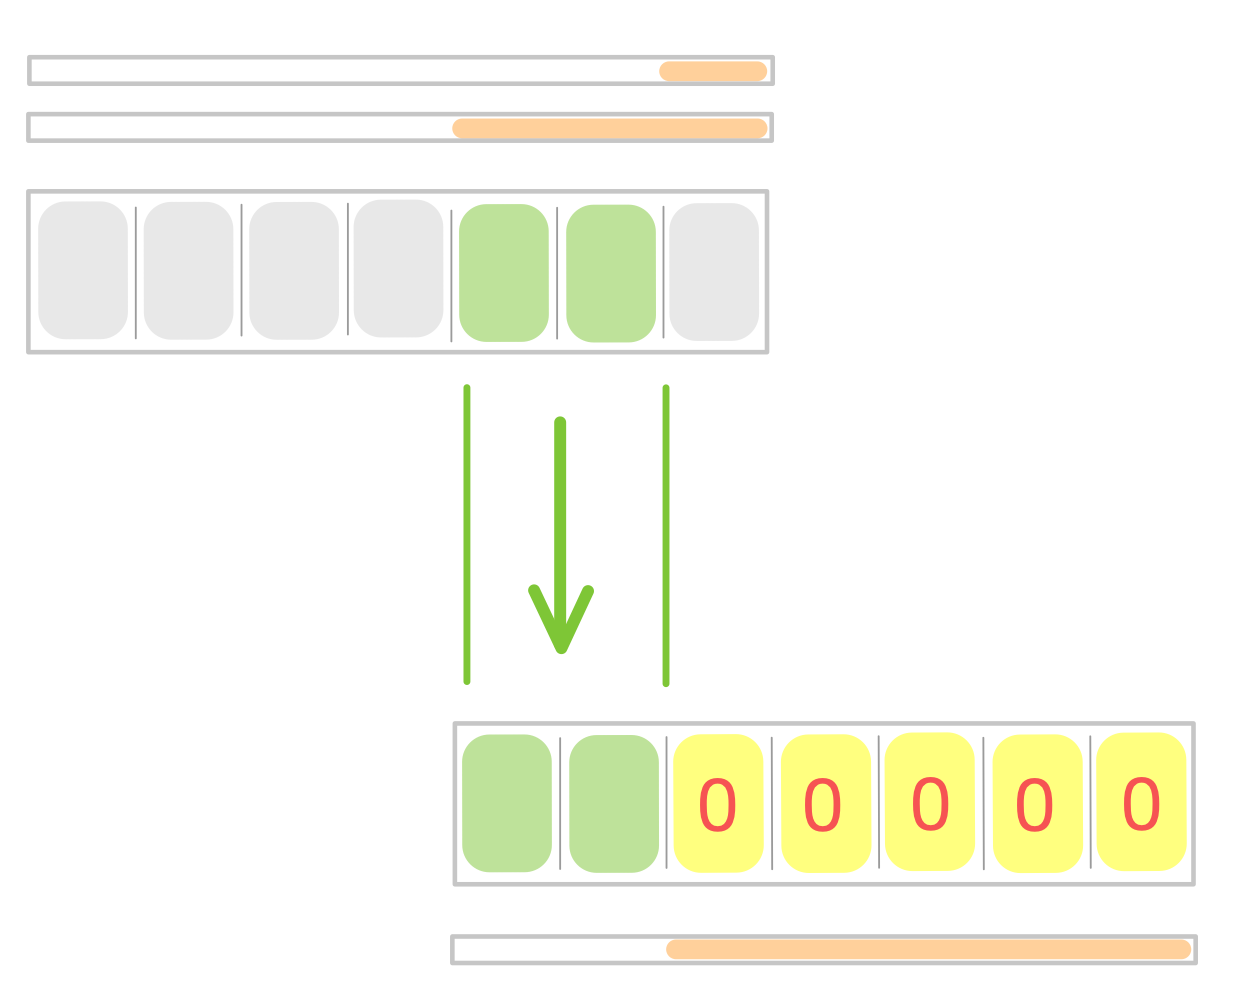
\includegraphics[width = 0.4\textwidth]{drawing/1_to_1_padded}
\label{fig: one partial to one padded}
\caption{Representation of the constraints implemented by $\oneToOnePadded$.}
\end{figure}